\documentclass{article}
\usepackage[utf8]{inputenc}
\usepackage[T1]{fontenc}
\usepackage{graphicx}
\usepackage{hyperref}
\usepackage{geometry}
\geometry{margin=1in}

\title{BUXUS}
\date{Encyclopaedia Britannica (1771)}

\begin{document}
\maketitle

\section*{Historical source}
\textbf{Entry ID:} \texttt{entry-buxus-2250} \\
\textbf{Volume ID:} 144133901 \\
\textbf{Character Count:} 579

\subsection*{Extracted Text}
BUXUS, in botany, a genus of the monocina terrandia elids. The calix of the male coaffins of three leaves; and the crotilla has two petals: The calix of the fo- male has four leaves; the petals are three; it has three flyily, and the copfila has three cells containing two feeds. There is but one species, viz, the fampevi-rens, or box-tree, a native of Britain. A decdition of the leaves and wood has been recommended as a powerful fiducifie; but is not now used by prestitioners. The wood is of a hard clole texture, and is greatly used by mechanics for toßls of various kinds.



\section*{Source record}
\begin{itemize}
\item \textbf{Dataset:} \texttt{NationalLibraryOfScotland/encyclopaedia\_britannica\_illustrated}
\item \textbf{Dataset Revision:} \texttt{309f765b1ecc83e0a7f7762e44b4a927a7555443}
\item \textbf{Page ID:} \texttt{britannica:309f765b1ecc83e0a7f7762e44b4a927a7555443:train:2250} \\
  \textbf{Filename:} \texttt{page-2250-75315f455009.jpg} \\
  \textbf{Row Index:} 2250 \\
  \textbf{SHA256:} \texttt{75315f45500988da...}
\end{itemize}

\begin{figure}[h]
\centering
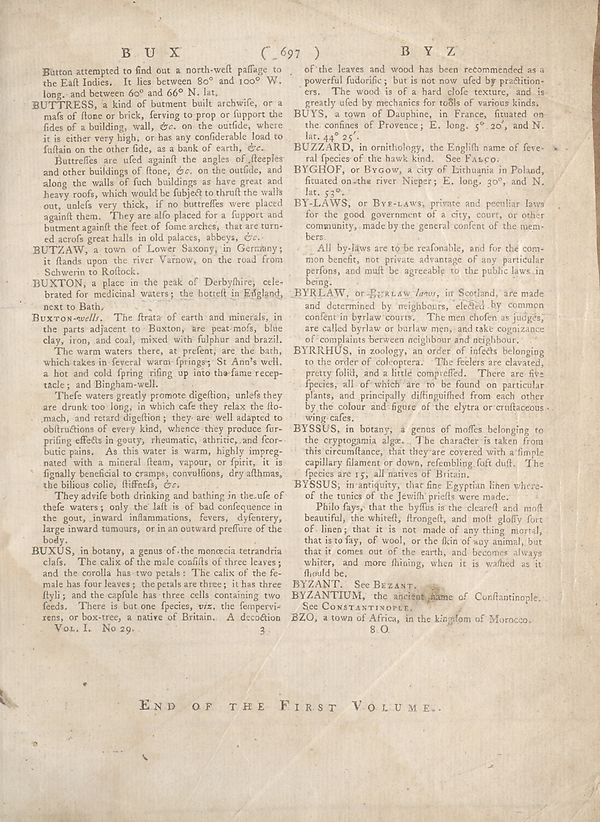
\includegraphics[width=0.85\textwidth]{../scans/page-2250-75315f455009.jpg}
\caption*{Source scan: \texttt{page-2250-75315f455009.jpg}}
\end{figure}

\end{document}
